\chapter{Introduction}
\label{ch:introduction}

\noindent Machine learning (ML) has become a central pillar of modern technology, powering applications in a multitude of fields such as healthcare~\citep{kotropoulos2009linear,sousa2009ordinal, challen2019artificial,guan2020bounded, mozannar2020consistent}, finance~\citep{9260038}, and transportation~\citep{ghodsi2021generating, tselentis2023usefulness}. These systems enable healthcare providers to diagnose diseases more accurately, financial institutions to tailor credit offers, and autonomous vehicles to navigate roads safely. Yet, as ML models increasingly transition from research environments to real-world settings, their reliability is under intensified scrutiny. As the stakes grow, so does the potential harm if models behave unexpectedly~\citep{amodei2016concrete, wiens2019no}: incorrect diagnoses can lead to life-threatening medical decisions, biased lending systems can exacerbate social inequities, and errors in autonomous driving technology can pose immediate safety hazards. These risks are further magnified by the complexity of large-scale data pipelines~\citep{pervaiz2019examining} and the often opaque nature of modern ML algorithms, which can make errors difficult to predict or detect. In addition, various industries are grappling with evolving regulatory and ethical standards~\citep{lo2020ethical, yaghini2024regulation} that demand greater accountability and transparency. 

Motivated by these risks, researchers and practitioners have begun to prioritize methods that enhance model trustworthiness and transparency. This has led to the emergence of the field of \textit{trustworthy machine learning}~\citep{li2023trustworthy}. Trustworthy machine learning aims to ensure that models not only excel at predictive performance but also uphold principles of reliability, fairness, privacy, accountability, as well as safety and security. It encompasses subfields dedicated to these goals, such as \textit{robust machine learning}~\citep{szegedy2013intriguing, papernot2017practical, rahimian2022frameworks}, which focuses on creating models resilient to variations in data distributions and adversarial inputs; \textit{fairness and bias mitigation}~\citep{hardt2016equality, mehrabi2021survey}, which aims to detect and reduce inequities that arise when data or algorithms systematically disadvantage certain groups; \textit{explainable or interpretable machine learning}~\citep{chen2019looks, rudin2019stop}, which seeks methods and frameworks to make complex model reasoning understandable to humans; and \textit{privacy-preserving techniques}~\citep{dwork2014algorithmic, abadi2016deep}, including differential privacy and federated learning, that protect sensitive information while enabling effective model training. Taken together, these subfields represent a concerted effort within the ML community to manage risks, fulfill ethical obligations, and promote transparent, accountable systems that reliably support high-stakes decisions in real-world contexts.

While each of these subfields provides essential guarantees to establish different notions of trust, they all share a dependence on a more fundamental capability: \textit{knowing the limits of a model's predictions}. A system cannot be considered truly robust, safe, or accountable if it cannot also signal when its conclusions are likely to be wrong. Consequently, a key challenge in making ML systems more reliable lies in \textit{quantifying uncertainty}~\citep{gal2016uncertainty, hullermeier2021aleatoric, gawlikowski2023survey}. Classical supervised learning methods often assume that models should output a single best prediction without any mechanism for indicating when this prediction might be wrong. In reality, however, uncertainty is an integral component of most prediction tasks. For instance, models trained on limited or noisy data can become overconfident in their predictions~\citep{guo2017calibration}, leading to harmful outcomes when deployed. This becomes especially clear when we consider high-stakes scenarios. Consider an autonomous vehicle navigating in dense fog or heavy rain: if the visual input is degraded, a well-calibrated uncertainty estimate can prompt the vehicle to slow down or safely stop rather than make an overconfident and potentially dangerous decision. In healthcare, a diagnostic model uncertain about whether a tumor is benign or malignant can flag the case for further review by a radiologist instead of issuing a definitive but incorrect diagnosis. In financial services, a model assessing loan applications can defer borderline cases to a human analyst if uncertainty is high, reducing the risk of unjust denials due to atypical applicant profiles. Consequently, techniques for quantifying and managing uncertainty are crucial to safe and responsible model deployment. These techniques can inform decisions about when a model is trustworthy enough to act on, when human oversight or additional information might be needed, and how to handle model predictions that are at high risk of being incorrect.

\begin{figure}[t]
    \centering
\begin{tikzpicture}[node distance=1cm,auto]
    \node[draw, thick, align=center] (x) {Input $x$};
    \node[right=of x, draw, thick, align=center] (f) {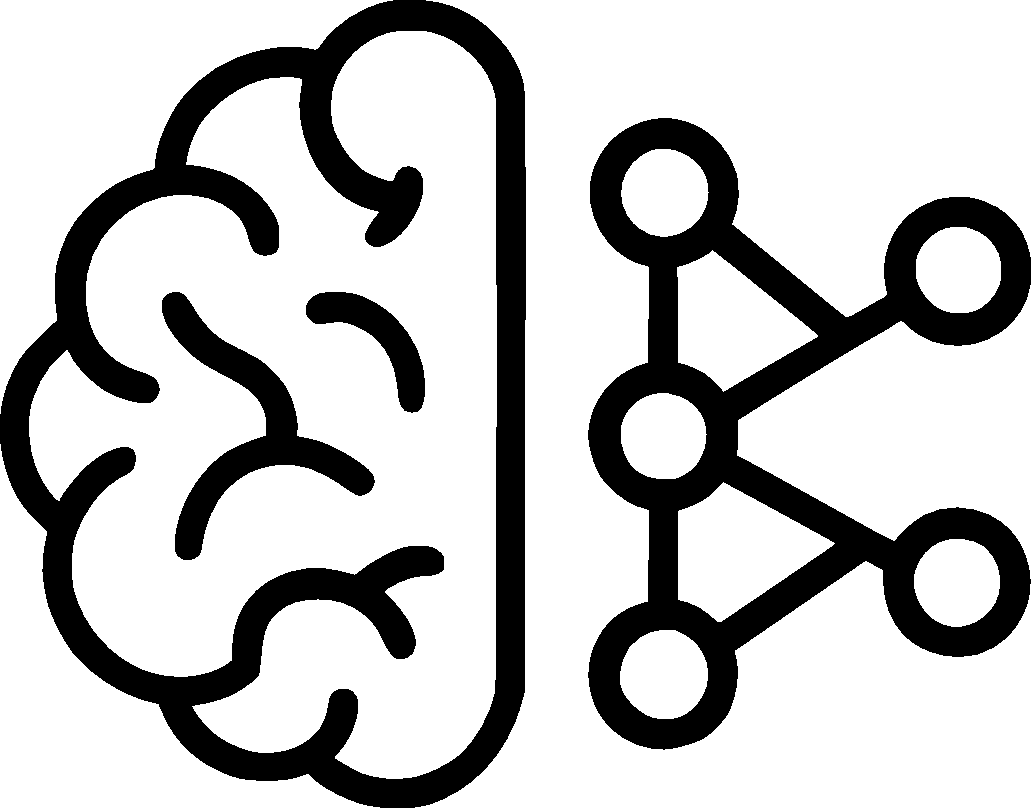
\includegraphics[width=45pt]{figs/model.pdf}\\ML Model $f$};
    \node[right=of f, draw, thick, align=center] (y) {Output $\hat{y}$};
    \draw[->, thick] (x) -- (f);
    \draw[->, thick] (f) -- (y);
    \node[below=of f, draw, thick, align=center, yshift=-15pt] (unc) {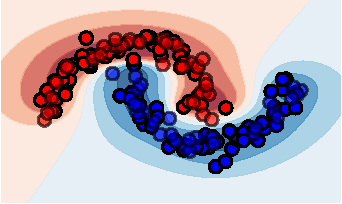
\includegraphics[width=80pt]{figs/gen_noborder.pdf}\\Uncertainty $p(y|x)$};
    \draw[->, thick] (x) to [out=270, in=90] (unc);
    \draw[->, thick] (f) to [out=270, in=90] (unc);
    \draw[->, thick] (y) to [out=270, in=90] (unc);
    \node[right=of y, diamond, draw, thick, align=center, fill = blue!25, xshift=30pt, yshift=-70pt] (pred) {Predict?};
    \draw[->, thick] (unc) to [out=0, in=180] (pred);
    \draw[->, thick] (y) to [out=0, in=180] (pred);
    \node[above=of pred, draw, Green, thick, align=center] (acc) {Return $\hat{y}$};
    \node[below=of pred, draw, red, thick, align=center] (rej) {Reject $\bot$};
    \draw[->, thick, Green] (pred) -- node[right] {Yes} (acc);
    \draw[->, thick, Red] (pred) -- node[right] {No} (rej);
    \end{tikzpicture}
    \vspace{10pt}
    \caption[Overview of the selective prediction pipeline.]{\textbf{Overview of the selective prediction pipeline}. Given an input \(x\), the model \(f\) produces a prediction \(\hat{y}\) along with an uncertainty estimate \(p(y|x)\). A selection function decides whether to return \(\hat{y}\) or reject with \(\perp\) based on the uncertainty.}
    \label{fig:selp_overview}
\end{figure}

Once reliable uncertainty estimates are available, the key challenge becomes translating them into principled actions. Decision theory offers a rich toolkit—ranging from Bayesian risk minimization to distribution-robust optimization—for choosing actions that balance expected utility against worst-case losses when outcomes are uncertain~\citep{berger2013statistical,rahimian2022frameworks}. In the supervised-learning setting, one of the most effective ways to operationalize this balance is to endow a model with an explicit \emph{reject option}: when the predicted probability of error exceeds a user-defined risk tolerance, the model abstains and defers the case to a downstream process such as a human expert, a more powerful model, or additional data collection~\citep{bartlett2008classification,geifman2017selective}. This paradigm—variously termed selective prediction, confidence-based abstention, or classification with a reject/abstain option—has seen growing adoption in high-stakes domains because it couples predictive performance with an actionable safeguard. Central to our work is precisely this concept of \textit{selective prediction} (SP, see Figure~\ref{fig:selp_overview})~\citep{chow1957optimum,el2010foundations}—an approach that allows the system to self-diagnose when it is likely to err and to withhold a decision rather than commit to a potentially harmful action. By integrating uncertainty estimates with abstention mechanisms, SP provides a formal pathway for aligning model behavior with real-world risk constraints, thereby transforming raw uncertainty into concrete, auditable decision rules that enhance safety and trustworthiness.

\vspace{15pt}
\section{Thesis Contributions}
\label{sec:contrib}

The overarching theme of this thesis is to embed uncertainty quantification at the heart of trustworthy machine learning (ML) systems. Central to our approach is the concept of selective prediction~\citep{chow1957optimum,el2010foundations}—which gives a model the option to abstain from making predictions it deems too risky. In this thesis, we make multiple contributions to this field. In short, we (i)~propose a new selective classification method based on ensembling intermediate models obtained from a single training run; (ii)~investigate the connection between selective prediction and differential privacy; (iii)~derive and analyze the key quantities that govern optimal selective prediction performance; and (iv)~study the effect of adversaries on the selective prediction pipeline. Below is an extended roadmap of how these ideas interconnect to form the core narrative of this thesis.

Before diving into the main contributions, we begin by laying the groundwork for what it means to \emph{measure} and \emph{manage} uncertainty in ML. This includes surveying classical approaches to calibrating confidence, examining how confidence estimates can fail in practice, and discussing why selectively rejecting uncertain inputs is an effective tool for mitigating high-impact errors. We highlight how uncertainty quantification (UQ) underpins reliable decision-making by offering interpretable confidence estimates, supporting risk-aware actions, and enabling resource-efficient deployment. Selective prediction is introduced as a natural downstream application of UQ—transforming uncertainty into a concrete decision to abstain when confidence is low. We emphasize the importance of calibration, robustness to distribution shift, and cost-aware thresholding, as well as the challenges that arise in deploying selective systems under real-world constraints. This background frames selective prediction not just as a technique, but as a paradigm for aligning model behavior with reliability objectives in safety-critical settings.

One of the most successful methods for uncertainty quantification we discuss is \emph{deep ensembling}~\citep{lakshminarayanan2017simple}, which estimates predictive uncertainty by training multiple models on different data subsets or with varying initializations. While ensembles are highly effective, their reliability typically improves with the number of members—making them computationally expensive at scale and difficult to deploy in resource-constrained or production environments. Motivated by this limitation, we ask whether a model’s \emph{training trajectory} can serve as a lightweight and scalable alternative for boosting selective prediction performance. Rather than modifying the model’s architecture or primary loss function, we demonstrate that signals extracted from intermediate checkpoints during training allow the model to self-diagnose its own likely points of failure. This yields a simple yet powerful abstention mechanism that can be applied post-hoc to any trained model with saved checkpoints—sidestepping the cost of full ensembles while retaining much of their reliability benefit. Moreover, this method is fully complementary to existing selective prediction approaches: it can be used to enhance any existing selector by providing an additional, trajectory-informed signal without interfering with the model’s original design or training objective.

Having demonstrated its practical utility, our training-dynamics-based approach also enables synergies with broader areas of trustworthy machine learning, making it especially well-suited for settings that demand the responsible deployment of AI. Because our approach merely observes the training process without interfering with it, it inherits a crucial compatibility with privacy-preserving learning: under the post-processing property of differential privacy (DP)~\citep{dwork2006calibrating}, operations applied after training do not compromise privacy guarantees. This makes our checkpoint-based method an attractive solution for \emph{uncertainty quantification in privacy-sensitive contexts}. We therefore turn next to exploring how selective prediction methods behave under strict privacy constraints. Many real-world applications demand that model training preserve the confidentiality of sensitive data, and DP is a gold standard for ensuring this. In this part of the thesis, we show how conventional selective prediction techniques—especially those reliant on ensembling—can amplify privacy risks or degrade under DP noise. In contrast, our training-dynamics-based approach proves particularly robust. This investigation also surfaces a deeper challenge: classical performance metrics often entangle improvements in overall model utility---a quantity which changes under varying privacy levels---with improvements in model uncertainty. To isolate uncertainty quality, we propose a new evaluation framework that enables a more faithful measurement of selective prediction performance in the presence of DP noise, capturing trade-offs between privacy, utility, and abstention coverage more effectively.

Studying privacy is a compelling example of responsible AI deployment—one that comes with an inherent utility trade-off and underscores the importance of evaluating selective prediction in scenarios where the base model's accuracy varies. The empirical and conceptual shortcomings revealed in this study therefore motivate a deeper interrogation of what actually determines selective prediction quality and performance. To that end, we study the \emph{selective-classification gap}, which corresponds to the deviation between a model's realized accuracy–coverage curve---the most commonly used evaluation metric in selective prediction---and a perfect-ordering upper bound established in our privacy work. We show that this gap can always be decomposed into five interpretable components: Bayes noise, approximation error, ranking error, statistical noise, and a miscellaneous term that captures optimization mishaps and distribution shift. The resulting finite-sample “error budget” clarifies which levers matter most at different coverage levels: increasing capacity or distilling from a stronger teacher shrinks the approximation term, additional or repeated labels dampen Bayes noise, larger validation sets reduce statistical fluctuations, and shift-aware training tackles the miscellaneous residue. Crucially, the analysis shows that monotone post-hoc calibration—long a default remedy for miscalibration—cannot touch the ranking term because it preserves the ordering of scores; progress therefore requires methods that can \emph{re-rank} predictions. By quantifying why and where models fall short of the oracle, this framework establishes principled targets for future algorithmic improvements.

Ultimately, claims of responsible AI deployment cannot simply be asserted by platform developers—they must be subject to external auditability. This naturally raises a critical question: can uncertainty quantification itself be gamed, especially in adversarial settings where the model operator cannot be fully trusted? In particular, the selective-classification gap analysis assumes that deviations from optimal performance stem from benign sources—such as modeling limitations or statistical fluctuations—not from active manipulation. Yet, in practice, the very mechanisms designed to improve reliability can themselves be exploited. This realization naturally leads us to investigate whether uncertainty, long viewed as a desirable and protective property in machine learning systems, might also be used \emph{maliciously}. Surprisingly, we find that confidence estimates can be easily deliberately manipulated to increase uncertainty in targeted input regions or for specific user groups, thereby covertly denying service while maintaining strong overall performance. These subtle attacks are difficult to detect because the system continues to perform well on aggregate metrics, even as it systematically disadvantages certain users. To counter this threat, we propose a verifiable inference mechanism that audits reported confidence and ensures that abstentions reflect genuine uncertainty. This work highlights a crucial lesson: secure and trustworthy ML requires not only sound estimation procedures, but also safeguards that ensure the integrity and authenticity of uncertainty itself.

\section{Thesis Statement}
\label{sec:contrib}

This leads us to the central thesis statement:

\boxedblock{
This thesis advances selective prediction—a model's ability to abstain when uncertain—as a cornerstone of trustworthy machine learning. Crucially, we observe that uncertainty can be effectively inferred from the inherent dynamics of the training process, rather than being retrofitted through costly modifications to the model or its training procedure. This approach provides a more direct path to robust selective prediction, which strengthens our ability to trust machine learning outputs. Consequently, because it preserves the integrity of the original training pipeline, this method is fundamentally more compatible with the principles of responsible ML deployment, enhancing crucial aspects such as differential privacy and model robustness against untrusted parties.
}

\section{Thesis Outline}
\label{sec:outline}

We summarize the contributions this thesis makes below:
\begin{itemize}
    \item \textbf{In Chapter~\ref{ch:background}}, we present background concepts crucial for understanding reliable decision-making in machine learning. We cover established approaches to modeling uncertainty, describe how predictive confidence is estimated, and discuss the rationale for selective prediction as a way to ensure safety by rejecting high-risk inputs. We also examine how confidence calibration underlies many of these techniques, enabling models to produce uncertainty estimates aligned with true error rates.

    \item \textbf{In Chapter~\ref{ch:sptd}}~\citep{rabanser2022selective}, we investigate how one can implement selective prediction by examining a model’s evolution throughout training, focusing on signals that emerge when predictions change or stabilize. We show that, by studying these signals, it is possible to determine which data points the final model is likely to misclassify. This perspective allows for a mechanism that rejects uncertain inputs without modifying the model’s architecture or primary optimization objective. The approach is adaptable to various tasks and domains, since it only requires access to intermediate training outputs.

    \item \textbf{In Chapter~\ref{ch:sptd_dp}}~\citep{rabanser2023training}, we delve into the interplay between selective prediction and differential privacy. We analyze how injecting random noise during training—an essential requirement for protecting sensitive data—can adversely affect a model's confidence estimates, reducing the reliability of conventional selective predictors. We examine why certain methods become less effective or more vulnerable under privacy constraints and propose refinements that leverage multiple training snapshots or other strategies to maintain robust performance. We also suggest novel evaluation metrics that better reflect how both privacy and reliability goals are being balanced.

    \textbf{In Chapter \ref{ch:sc_bounds}}~\citep{rabanser2025what}, we take a principled look at what governs how close a selective predictor can come to its oracle ideal. We formalize the \emph{selective-classification gap}—the deviation between a model’s accuracy–coverage curve and the perfect-ordering frontier—and derive the first finite-sample decomposition that attributes this gap to five interpretable error sources: Bayes noise, approximation limits, ranking imperfections, statistical fluctuations, and miscellaneous factors such as optimization error or distribution shift. The resulting “error budget’’ clarifies which levers (e.g., capacity, ranking-aware calibration, additional labels, or shift-robust training) most effectively shrink the gap at different coverage levels. We further prove that monotone post-hoc calibration cannot close the ranking term, motivating algorithms that can re-order confidence scores, and we validate the theory on tasks ranging from synthetic two-moons to large-scale vision benchmarks.

    \item \textbf{In Chapter~\ref{ch:conf_guard}}~\citep{rabanser2025confidential}, we highlight a potential adversarial threat in selective prediction systems: malicious entities can artificially suppress model confidence in targeted regions or for specific groups while retaining high performance elsewhere. This tactic allows an attacker to deny services or introduce bias under the pretense of uncertainty. We describe how such manipulation can be carried out, and we develop a strategy to detect and deter artificially induced low confidence. Central to this solution is the need for mechanisms that can verify confidence values or otherwise ensure that the model's abstentions are genuinely driven by uncertainty rather than deliberate manipulation.

    \item \textbf{In Chapter~\ref{ch:conclusion}}, we conclude by summarizing the contributions of the thesis and highlighting future directions. We reflect on open research questions in areas such as adaptive calibration, reliability and uncertainty in large models, new forms of adversarial threats, and privacy-preserving learning. We also consider the broader implications of adopting selective prediction at scale, including ethical considerations in sensitive or high-stakes applications.
\end{itemize}

\paragraph{Non-Thesis Research} Publications on which I have worked during my Ph.D. which are excluded from this thesis include (in chronological order):

\begin{itemize}
    \item \citet{dziedzic2022p}: \bibentry{dziedzic2022p}.\\[10pt]

    $p$-DkNN is a method for producing statistically grounded uncertainty estimates in neural networks by analyzing the similarity structure of intermediate representations and computing $p$-values for predictions. This allows us to improve the trade-off between rejecting OOD inputs and maintaining accuracy on in-distribution data. The approach is scalable, theoretically connected to Neyman–Pearson classification, and robust enough to make adversarial attacks require semantically meaningful changes.
    
    \item \citet{rabanser2022intrinsic}: \bibentry{rabanser2022intrinsic}.\\[10pt]
    In this work we introduce intrinsic anomaly detection for multivariate time series, focusing on identifying unexpected changes in a system’s state relative to its environment. We formalize the problem, release relevant datasets, and propose unsupervised methods—combining domain-adversarial and representation learning—that distinguish true anomalies from environment-driven changes.
    
    \item \citet{franzese2023robust}: \bibentry{franzese2023robust}.\\[10pt]
    Collaborative ML can improve models from distributed data but is vulnerable to malicious servers reconstructing client data and malicious clients corrupting updates. This work introduces a peer-to-peer learning framework that secures against untrusted servers and is robust to malicious clients by adapting robust aggregation methods to this setting. The approach is computationally efficient and scales to millions of parameters and hundreds of peers.
    
    
    \item \citet{pouget2025suitability}: \bibentry{pouget2025suitability}.\\[10pt]
    The suitability filter is a framework for detecting when a deployed model’s accuracy on unlabeled user data has degraded beyond an acceptable margin, without needing ground-truth labels. It works by comparing model output–based suitability signals from test and user data via statistical hypothesis testing. Experiments show it reliably flags performance drops caused by covariate shift in safety-critical settings.
    
    \item \citet{rabanser2025gatekeeper}: \bibentry{rabanser2025gatekeeper}.\\[10pt]
    Gatekeeper is a new loss function for cascade setups that fine-tunes smaller models to confidently handle easy tasks while deferring harder ones to larger models. It balances performance and deferral accuracy without changing model architectures, and works across diverse tasks and domains. Our experiments on multiple architectures and modalities show substantial improvements in deferral performance.
    
    \item \citet{jiang2025cascadia}: \bibentry{jiang2025cascadia}.\\[10pt]
    Cascadia is a new framework for serving large language model (LLM) cascades that balances speed and answer quality by jointly optimizing routing strategies and system deployment. Using a bi-level optimization approach, it allocates resources and parallelism for different LLMs while adapting routing to workload characteristics. Our experiments show it outperforms existing approaches, delivering up to 4× tighter latency SLOs and 5× higher throughput without sacrificing quality.
\end{itemize}